Immaginiamo di avere una sola specie chimica nello stato liquido.

\begin{figure}[htp]
    \centering
    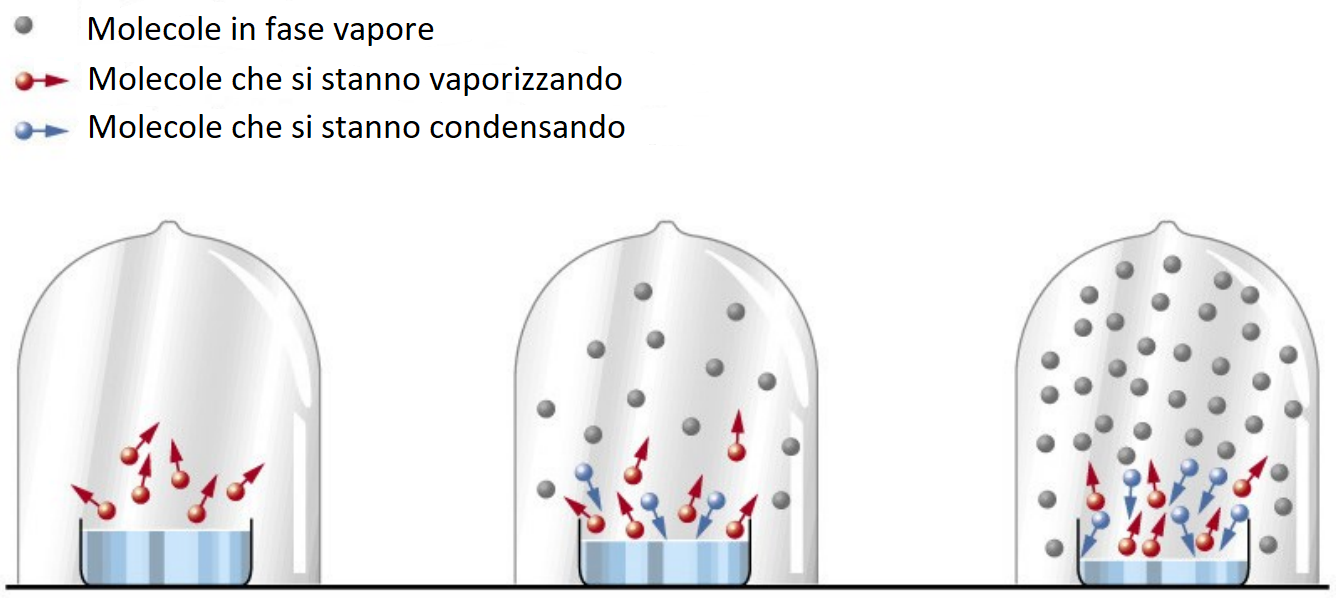
\includegraphics[width=15cm]{immagini/campana_di_vetro}
\end{figure}

Sarà opportuno racchiudere il contenitore con una campana di vetro in cui è preventivamente fatto il vuoto in modo da non avere particelle diverse da quello del liquido.

Si lascio poi evaporare, o meglio si attende fino a quando si stabilisce un equilibrio, in quanto alcune particelle del liquido ne abbandonano la superficie per passare in fase vapore. Altre particelle nella fase vapore tenderanno invece a tornare nella fase liquida e ad un certo punto si raggiunge un equilibrio in cui la pressione delle particelle del liquido che sono passate dalla fase liquida a quella vapore è detta "\textbf{tensione di vapore}" o "pressione di vapore". Essa sarà la pressione esercitata sulle pareti della campana di vetro, in quanto avendo fatto il vuoto non ci sarà altra pressione.

Il fenomeno di passaggio da uno stato all'altro delle particelle dipende dalla temperatura, per cui a temperatura costante si avrà pressione costante dovuta solo alle particelle in fase vapore.

\vspace{0.2cm}\E chiaro che questo è un equilibrio dinamico: continuamente delle particelle che stanno in fase vapore tornernanno a far parte della fase liquida e viceversa dalla superficie del liquido altre particelle passeranno allo stato di vapore, ma nell'istante in cui si raggiunge tale equilibrio la tensione di vapore non cambia.

Inoltre il numero di particelle che abbandona la fase liquida per passare alla fase di vapore cresce all'aumentare della temperatura

\hspace{0.5cm}\begin{minipage}{0.5 \textwidth}
    \begin{figure}[H]
        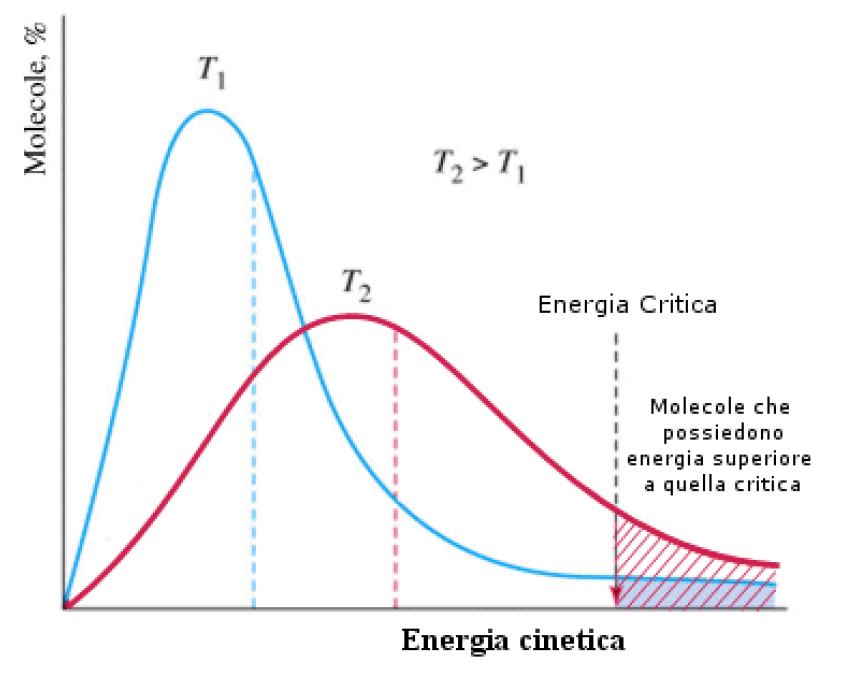
\includegraphics[width=7cm]{immagini/energie_fase_liquida.png}
    \end{figure}
\end{minipage}
\begin{minipage}{0.4 \textwidth}
\vspace{0.5cm}Dal grafico si evince che l'andamento a due diverse temperature mostra un picco nella percentuale di molecole che possiede una data energia e all'aumentare della temperatura tale picco si sposta a più alta energia e tende ad appiattirsi.
\end{minipage}

\vspace{0.2cm}Deduciamo che la percentuale di molecole ad alta energia è maggiore all'aumentare della temperatura, e scciome le particelle che riescono a passare dalla fase liquida a quella vapore sono quelle a più alta energia ne segue che aumenta il numero di quest'ultime.

\hspace{0.5cm}\begin{minipage}{0.5 \textwidth}
    \begin{figure}[H]
        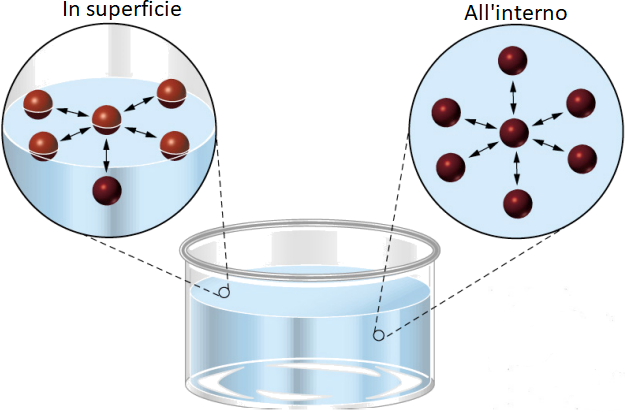
\includegraphics[width=7cm]{immagini/interazioni_nel_liquido.png}
    \end{figure}
\end{minipage}
\begin{minipage}{0.5 \textwidth}
    \begin{figure}[H]
        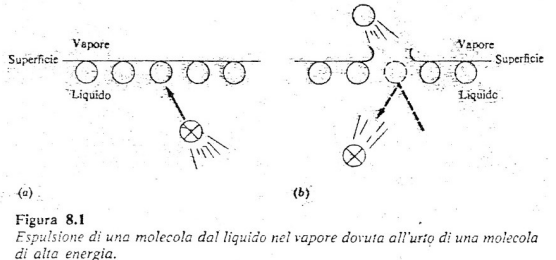
\includegraphics[width=7cm]{immagini/espulsione_particelle.png}
    \end{figure}
\end{minipage}

\vspace{0.3cm}Va da ricordare che all'interno del liquido qualunque particella è sottoposta a delle interazioni in tutte le direzioni. Viceversa sulla superficie del liquido la particella è sottoposta solo ad alcune di queste interazioni perché alcune mancano.

Si può dire che le particelle che passano da liquido a vapore vengano in qualche modo spinte dalle particelle interne con urti.

\vspace{0.2cm}Definiamo poi \textbf{temperatura di ebollizione} per qualunque sostanza la temperatura alla quale la tensione di vapore di tale sostanza eguaglia la pressione atmosferica.

\hspace{0.5cm}\begin{minipage}{0.5 \textwidth}
    \begin{figure}[H]
        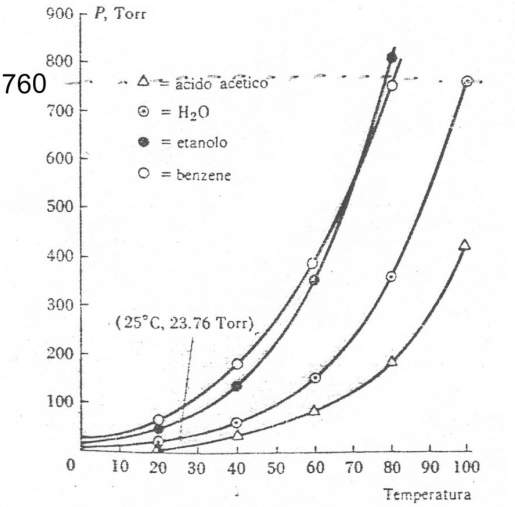
\includegraphics[width=7cm]{immagini/tensioni_di_vapore.png}
    \end{figure}
\end{minipage}
\begin{minipage}{0.4 \textwidth}
Notiamo dal grafico che la tensione di vapore dei diversi composti, a parità di temperatura, è diversa.

\vspace{0.2cm}Ad esempio a parità di temperatura l'acqua mostra una tensione di vapore più bassa di quella dell'etanolo o del benzene, ma più alta dell'acido acetico.
\end{minipage}
\E importante quindi capire perché composti diversi mostrino tensioni di vapore diverse a parità di temperatura.

A naso si potrebbe dire che la massa delle particelle determinerà questa caratteristica, per cui particelle con massa maggiore eserciteranno, a parità di temperatura, una tensione di vapore minore rispetto quelle con massa minore, ma spesso non è così. Si vede anche nel grafico: il benzene C$_6$H$_6$ ha peso molecolare maggiore dell'acqua H$_2$O, ma a parità di temperatura ha tensione di vapore maggiore.

\begin{figure}[htp]
    \centering
    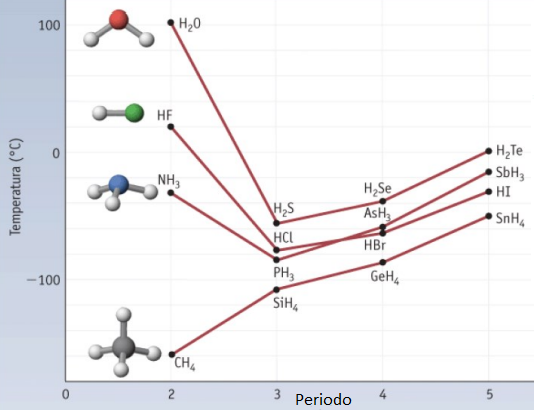
\includegraphics[width=12cm]{immagini/temperature_ebollizione.png}
\end{figure}